\chapter{Introduction}

Many scientific applications require far more computation or data storage than can be handled on a regular PC or laptop. For such applications, access to remote storage and compute facilities is essential. Unfortunately, there is not a single standardized way to access these facilities. There are many competing protocols and tools in use by the various scientific data centers and commercial online providers.

As a result, application developers are forced to either select a few protocols they wish to support, thereby limiting which remote resources their application can use, or implement support for all of them, leading to excessive development time.

Xenon is a library designed to solve this problem. It offers a simple, unified programming interface to many remote computation and data storage facilities, and hides the complicated protocol and tool specific details from the application. By using Xenon, the application developer can focus on the application itself, without having to worry about which protocols to support, resulting in faster application development.

% TODO examples of what you can do with it

\section{Purpose of this document}

This document aims to help users without much prior knowledge about Java programming and without much experience in using remote systems to understand how to use the Xenon library.

\section{Version information}

It is assumed that you are using one of the Ubuntu-based operating systems (I'm using Linux Lubuntu 14.10). Nonetheless, most of the material covered in this manual should be usable on other Linux distributions with minor changes. The manual is written to be consistent with Xenon release 1.1.1\footnote{For releases, see \url{https://github.com/NLeSC/Xenon/releases}}.


\section{Conceptual overview}

% TODO what is middleware




Xenon consists of three pillars: `credentials'\index{Xenon!pillars!credentials}, `files'\index{Xenon!pillars!files}, and `jobs'\index{Xenon!pillars!jobs}.
%
The credentials pillar contains functionality pertaining to credentials. Credentials (such as a name and password combination) are often required to gain access to files or to submit jobs.
%
The files pillar contains all functionality relating to files, such as creation, deletion, copying, reading, writing, obtaining a directory listing, etc.
%
Lastly, the jobs pillar contains functionality relating to jobs, e.g. submitting, polling, cancelling, etc.

% TODO explain the notion of files (files interface)
% TODO explain the notion of jobs (jobs interface)
% TODO explain the notion of credentials (credential interface)
% TODO explain the notion of adaptors

\begin{figure}[ht]
\centering
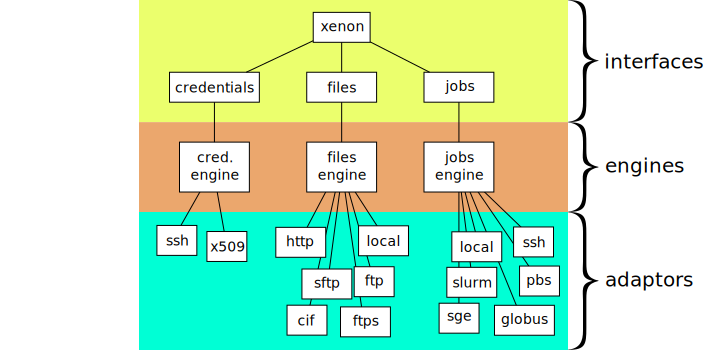
\includegraphics[width=1.0\columnwidth]{images/xenon-design}
\caption{\label{fig:xenon-design} Xenon is built on 3 pillars: `credentials'\index{Xenon!pillars!credentials}, `files'\index{Xenon!pillars!files} and `jobs'\index{Xenon!pillars!jobs}. Each pillar consists of an interface\index{Xenon!interface}, an engine\index{Xenon!engine}, and an adaptor\index{Xenon!adaptor}.}
\end{figure}
